\section{Results}

The total U.S. Resource is estimated to be between 3170 and 3845 TWh/yr (Table~\ref{table:totals}). Around 2/3 of the resource are in the Alaskan EEZ both due to the combination of a large area and large waves. The East Coast and West Coast EEZs are comparable (the former bein 11\% larger) but their resources are very different. The remote resource dominates the West Coast as the Pacific has consistently bigger waves than the Atlantic (in the northern hemisphere). However, strong westerly winds with a less developed sea state coalesce to generate strong local waves yielding a local resource that is 89\% larger than that in the West Coast.  The Caribbean has the smallest remote resource in part because only the northern boundary of the EEZ is exposed to the open ocean yielding a small area of integration. In this case the local resource is also larger than the potential resource. \note{I am terrible at describing tables, I wont be offended if you delete all this text.}

\begin{table}[ht]
  \centering
  \begin{tabular}{|c|c|c|c|c|}
    \hline
    Region & Remote & Local & Potential & Total \\
    \hline
    West Coast & 420 & 90 & 190 & 510 - 610 \\
    Hawaii & 290 & 10 & 90 & 300 - 380 \\
    East Coast & 110 & 170 & 210 & 280 - 320 \\
    Gulf of Mexico & 13 & 50 & 60 & 63-73 \\
    Alaska & 1040 & 960 & 1390 & 2000 - 2430 \\
    Puerto Rico & 6 & 11 & 26 & 17 - 32 \\
    \hline \hline
U.S. TOTAL & 1879 & 1291 & 1966 & 3170 - 3845 \\
\hline
  \end{tabular}
  \caption{Wave resource assessment results by region and totaled for the entire U.S. (all values in TWh/yr). The range in the total column indicates the sum of Remote+Local (lower value) and Remote+Potential (higher value). \note{We need to confirm these values again.}}
  \label{table:totals}
\end{table}

The large increase in resource in Hawaii is due in large part due to the exteneded area of integration. In the EPRI 2011 report the integration was performed at the 200 m isobath, which in the case of Hawaii is very close to shore due to the lack of continental shelf. In the present case, integration contour is extented to the EEZ which lies at 200 nmi in the Northern, Eastern, and Southern boundaries.

\begin{table}[ht]
  \centering
  \begin{tabular}{|c|c|c|c|}
    \hline
    Region 
    &
      \begin{tabular}{c}
        EPRI 2011 \\ {\it Remote Only} \\ $\mathrm{[TWh/yr]}$
      \end{tabular}
    &
      \begin{tabular}{c}
        New Total \\ TWh/yr
      \end{tabular}
    & \% Change \\
    \hline
    West Coast & 590 & 510 - 610 & -5 $\pm$10 \\
    Hawaii & 130 & 300 - 380 & +160 $\pm$30 \\
    East Coast & 240 & 280 - 320 & 25 $\pm$8 \\
    Gulf of Mexico & 80 & 63 - 73 & -15 $\pm$7 \\
    Alaska & 1570 & 2000 - 2430 & +40 $\pm$15 \\
    Puerto Rico & 30 & 17 - 32 & -20 $\pm$25 \\
    \hline \hline
    U.S. TOTAL  & 2640 & 3170 - 3845 & +33 $\pm$ 13 \\
    \hline
  \end{tabular}
  \caption{Wave resource totals compared to 2011 results (all values in TWh/yr).}
  \label{tab:total-compare}
\end{table}

\begin{figure}[ht]
  \centering
  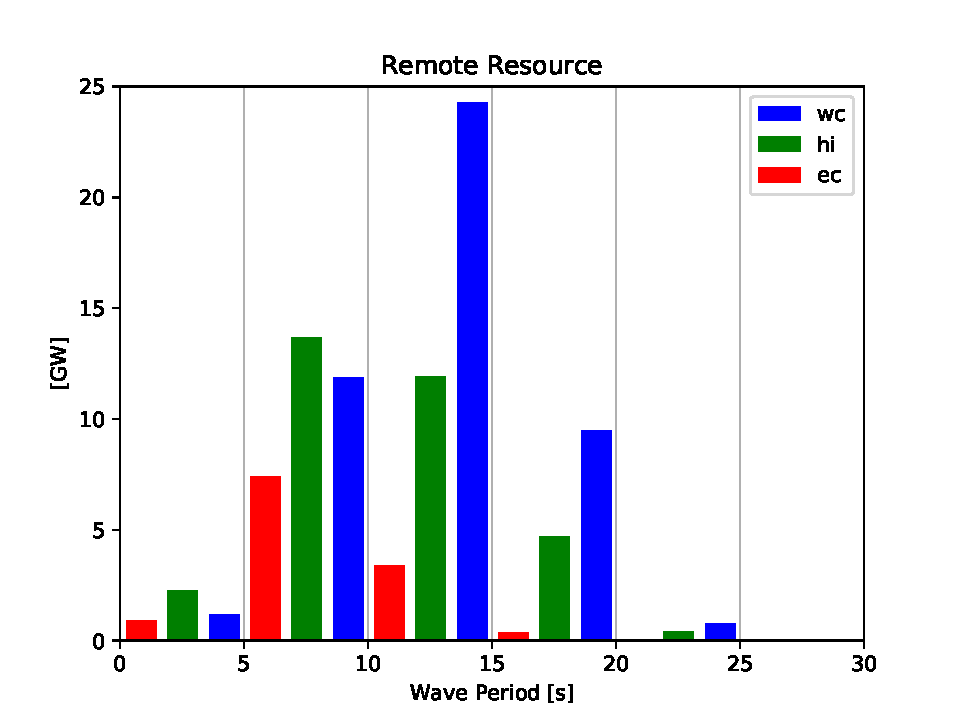
\includegraphics[width=\linewidth]{../fig/RemoteResource_Freq01.pdf}
  \caption{Remote resource contained in each wave period band (0-5 seconds, 5-10 seconds, etc.) for the west coast (wc), Hawaii (hi), and the east coast (ec).}
  \label{fig:remote-freq}
\end{figure}

\begin{figure}[ht]
  \centering
  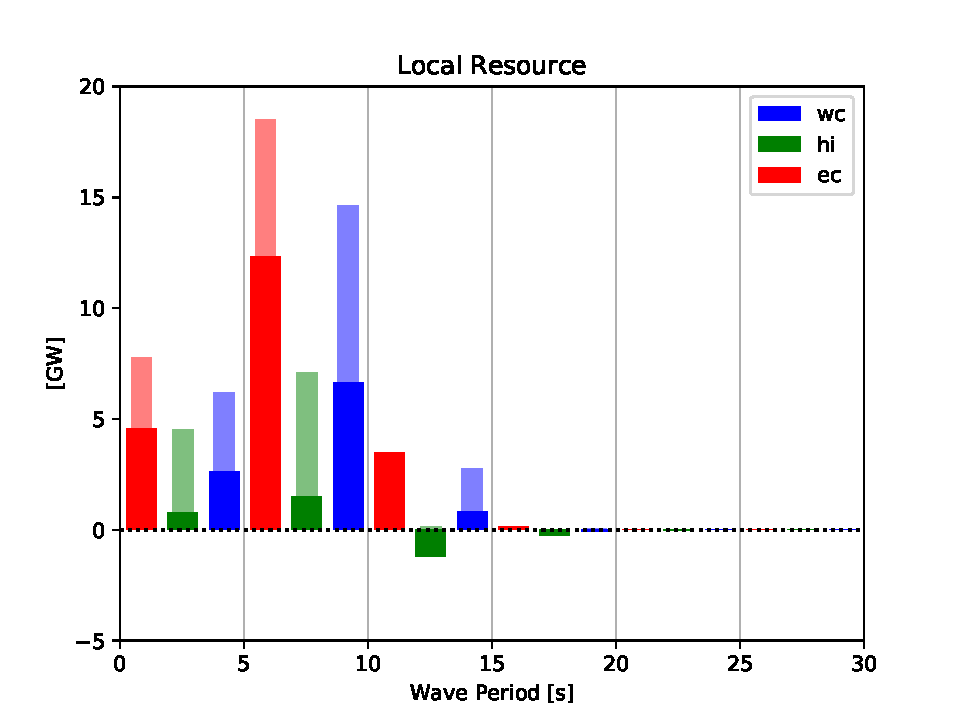
\includegraphics[width=\linewidth]{../fig/LocalResource_Freq01.pdf}
  \caption{Local (thick solid bars) and potential (narrow pale bars) resource contained in each wave period band (0-5 seconds, 5-10 seconds, etc.) for the west coast (wc), Hawaii (hi), and the east coast (ec).}
  \label{fig:remote-freq}
\end{figure}

\begin{itemize}
\item National total plus Regional/State-by-state breakdown of resource.
=======
\item \note{Levi: I would change the tag Puerto Rico for Caribbean or PR\&USVI}
\item National total plus Regional/State-by-state breakdown of resource. \textcolor{green}{We do not have the resolution to do the territorial waters accurately, they are just 3 nmi from shore in most cases.}
>>>>>>> clean-slate-ggm
\item Plots of ‘remote’ resource vs. distance from shore (Figure 5). ... How does this compare with local resource vs. distance from shore?
\item Remote resource vs. depth. Local resource vs. depth.
\end{itemize}


%%% Local Variables:
%%% TeX-master: "wave_res"
%%% End:
